% !TeX encoding = UTF-8
% !TeX spellcheck = en_GB
\section{CI/CD pipelines}
\paragraph{} To configure and execute our CI/CD pipeline we use GitHub Actions. We chose to use GH Actions because we were already using GitHub for our repository, and GH Actions provided a seamless integration in our workflow in GitHub. Furthermore, it was easy to set up, and the free plan was more than enough for our needs.

\paragraph{} We have configured two different variants of the pipeline: one that is executed when a PR is opened or updated, and one that is triggered on pushes to main, which, in practice, is only triggered on PR merges to main, since we never push directly to main. The tasks performed by the pipeline are as follows:
\begin{enumerate}
	\item \textbf{Build and test the application}: In this step we build the application, run the unit tests, UI test and end-to-end tests. The unit test are run during the building of the image, while the UI and end-to-end tests are each run by using a specially-crafted compose.yml file, which allows us to run the application, the database, and the UI or E2E tests simultaneously. We then instruct docker compose to use the exit code from the container executing the tests, which makes the pipeline fail if any of the tests has failed. This step is executed both when PR and opened or updated, and when a push is made to main.
	\item \textbf{Linting}: In this step we execute linters for our code and Dockerfiles, with the use of the third-party GH action "super-linter". If problems are detected, this part of the pipeline reports an error. This step is only executed when a PR is opened or updated.
	\item \textbf{Build and push image}: In this step, a production docker image is build and pushed to our image repository. This image will then be used on the deployment step. This step is only executed when a push is made to main. 
	\item \textbf{Create release}: In this step, a release is created on the GH repository, with the contents of the commit triggering the pipeline. This step is only executed when a push is made to main. 
	\item \textbf{Deployment}: In this step, our image is deployed to our server. To do so in a safe way, we have devised a deployment system which is triggered by a simple SSH login:
	\begin{itemize}
		\item In our VM we have an used called deploy. When someone logs in as this used, either by SSH or by using su, a script is executed. The person logging in cannot execute any other command other than the script, to prevent security issues should someone obtain the keys to the user. When the script finishes, the user is logged out.
		\item This script connects to GitHub and clones our "server-files" repository, and executes the script deploy.sh, which contains the deployment logic.
		\item This script then pulls the necessary images, including our image created on a previous step, and deploys them in the server. The script uses other files which are also stored on the same repository, such as a compose.yml, which specifies which images to use, and configuration files for f.e. grafana and prometheus.
		\item The scripts also use secrets, f.e to clone the repository from GH, pull the image, or to configure the app to properly connect to our database (which is not located on the VM). These variables are stored on text files on the server. In order to maximize security, these files are owned by root, and are only readable by root or by members of the group deployers (of which deploy is a member), which prevents them from being read by unauthorized users. The bash scripts then access these files and export them as environment variables, which then can be used where they are required.
	\end{itemize}
	In this step, we simply log to our server via SSH from GH Actions, which triggers the whole deployment procedure on the server. This step is only executed when a push is made to main. 
\end{enumerate}
During the execution of the pipeline we need to use some secrets, f.e. to SSH into our server. We use GitHub Secrets to store those.

\paragraph{} In figures \ref{fig:ci-push} and \ref{fig:ci-pr} the flow of the different steps can be seen, both in the case of a PR-triggered pipeline and in the case of a pipeline triggered by a push to main.

\begin{figure}[h]
	\centering
	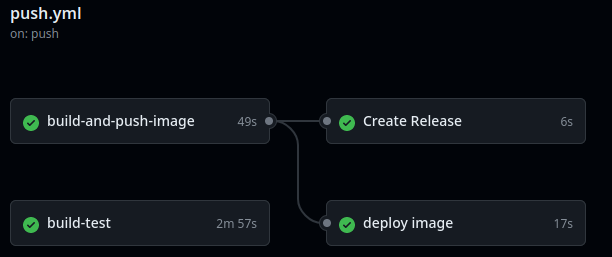
\includegraphics[width=0.75\textwidth]{ci-push.png}
	\caption{Diagram with the different steps executed by the pipeline on a push to main.}
	\label{fig:ci-push}
\end{figure}

\begin{figure}[h]
	\centering
	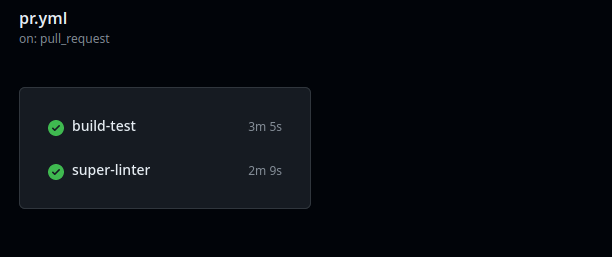
\includegraphics[width=0.75\textwidth]{ci-pr.png}
	\caption{Diagram with the different steps executed by the pipeline when a PR is opened or updated.}
	\label{fig:ci-pr}
\end{figure}

\paragraph{} We also use the Maintainability and Technical Debt estimation tool SonarCube, which provides us reports of our code quality directly in GitHub. However, this tool is managed in its own website, and it is not configured as part of GH Actions.

\subsection{Report compilation}
\paragraph{} We also have an additional GH Action, which is only triggered by pushes which modify files in the "report" subfolder. This action then compiles the \LaTeX project located in that subfolder and generates a PDF, which then commits to the "report/build" subfolder.